\subsubsection{Sequence Diagram - Module Quản lý tổ chức}

\begin{figure}[H]
    \centering
    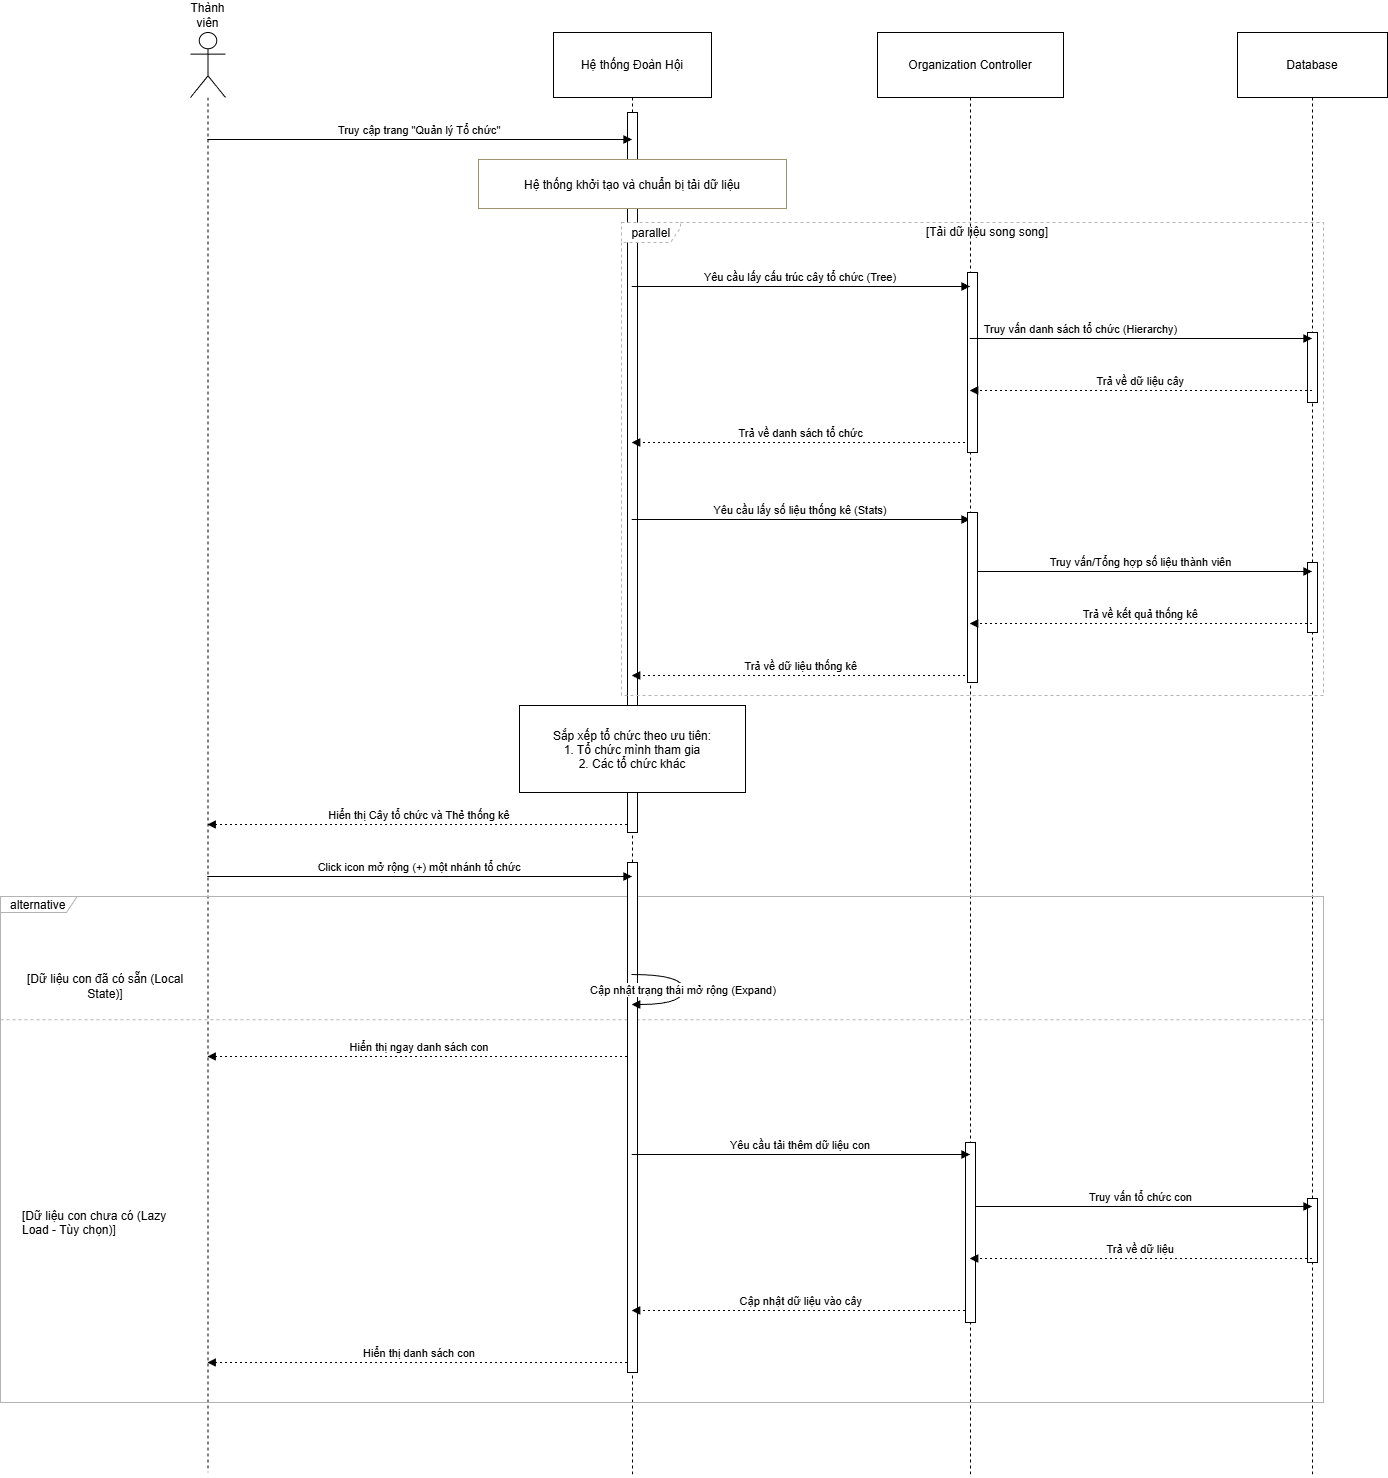
\includegraphics[width=1.0\textwidth]{Images/sequence-diagram/SQ04_organization_sequence.drawio .png} 
    \caption{Sequence Diagram - Luồng hoạt động của quản lý tổ chức }
    \label{fig:seq_org_tree}
\end{figure}
Quy trình hiển thị và tương tác với cấu trúc tổ chức (Organization Tree) là một trong những nghiệp vụ quan trọng, yêu cầu tốc độ phản hồi nhanh và trải nghiệm người dùng mượt mà. Biểu đồ tuần tự (Sequence Diagram) tại Hình \ref{fig:seq_org_tree} mô tả chi tiết luồng tương tác giữa Thành viên, Hệ thống Frontend và Backend Controller.
Quy trình xử lý được chia thành hai giai đoạn chính nhằm tối ưu hóa hiệu năng hệ thống:

\paragraph{Giai đoạn 1: Khởi tạo và Tải dữ liệu song song}
Khi người dùng truy cập vào trang quản lý, hệ thống không thực hiện các lệnh gọi API tuần tự mà sử dụng kỹ thuật \textbf{Parallel Processing} (Xử lý song song) để giảm thiểu tổng thời gian phản hồi (Total Response Time).
\begin{itemize}
    \item \textbf{Truy vấn cấu trúc cây (Tree Structure):} Hệ thống gửi yêu cầu đến \textit{Organization Controller} để lấy danh sách tổ chức phân cấp.
    \item \textbf{Truy vấn thống kê (Statistics):} Đồng thời, một luồng xử lý khác truy vấn số liệu tổng hợp về thành viên từ cơ sở dữ liệu.
\end{itemize}
Sau khi nhận đủ dữ liệu từ cả hai luồng, Frontend thực hiện thuật toán sắp xếp cục bộ (\textit{Client-side Sorting}). Các tổ chức mà người dùng đang là thành viên sẽ được ưu tiên hiển thị lên đầu danh sách (Priority 1), giúp người dùng tiếp cận thông tin quan trọng nhanh nhất.

\paragraph{Giai đoạn 2: Tương tác và Cơ chế Lazy Loading}
Để giảm tải băng thông và dung lượng bộ nhớ ban đầu, hệ thống áp dụng cơ chế \textbf{Lazy Loading} (Tải dữ liệu theo nhu cầu) cho các thao tác mở rộng nhánh cây:
\begin{enumerate}
    \item Khi người dùng kích hoạt mở rộng một nhánh tổ chức, hệ thống kiểm tra trạng thái dữ liệu cục bộ (\textit{Local State}).
    \item \textbf{Trường hợp Cache Hit:} Nếu dữ liệu nhánh con đã tồn tại, giao diện được cập nhật tức thì mà không cần gọi về Server.
    \item \textbf{Trường hợp Cache Miss:} Nếu dữ liệu chưa có, hệ thống mới gửi yêu cầu tải bổ sung (\textit{Fetch additional data}) tới Controller. Dữ liệu mới sau đó được cập nhật vào cây và hiển thị cho người dùng.
\end{enumerate}

Giải pháp này giúp hệ thống đảm bảo khả năng mở rộng tốt (Scalability) ngay cả khi số lượng tổ chức trong trường tăng lên hàng nghìn đơn vị, đồng thời duy trì trải nghiệm mượt mà cho người dùng cuối.